\documentclass[a4paper,12pt]{article}

\usepackage{graphicx}
\usepackage{caption}
\usepackage{subcaption}
\usepackage[utf8]{inputenc}
\usepackage[english,greek]{babel}

\title{Τεχνικές Βελτιστοποίησης - Εργασία 2}
\author{Ρουσομάνης Γεώργιος (ΑΕΜ: 10703)}
\date{Νοέμβριος 2024}

\begin{document}

\maketitle

\section*{Εισαγωγή}

Ο στόχος της παρούσας εργασίας είναι η ελαχιστοποίηση μιας συνάρτησης πολλών μεταβλητών χωρίς περιορισμούς με 
τη χρήση παραγώγων και η μελέτη της αποτελεσματικότητας διαφορετικών αλγορίθμων βελτιστοποίησης. Ειδικότερα,
η αντικειμενική συνάρτηση που θα εξεταστεί είναι:

\[
f(x, y) = x^5 e^{-x^2 - y^2}.
\]

Οι μέθοδοι που θα χρησιμοποιηθούν για την αναζήτηση του ελαχίστου περιλαμβάνουν:
\begin{itemize}
    \item \textbf{Μέθοδος Μέγιστης Καθόδου \selectlanguage{english} (Steepest Descent) }
    \item \textbf{Μέθοδος \selectlanguage{english} Newton}
    \item \textbf{Μέθοδος \selectlanguage{english} Levenberg-Marquardt}
\end{itemize}

Η κατεύθυνση καθόδου $d_k$ καθορίζεται διαφορετικά σε κάθε μέθοδο, ενώ το βήμα $\gamma_k$ μπορεί να επιλεχθεί
είτε σταθερό, είτε με ελαχιστοποίηση της $f(x_k + \gamma_k d_k)$, είτε βάσει του κανόνα 
\selectlanguage{english} Armijo. \selectlanguage{greek}
Σε κάθε επανάληψη, το νέο σημείο υπολογίζεται ως $x_{k+1} = x_k + \gamma_k d_k$
ενώ οι αλγόριθμοι τερματίζουν όταν $|\nabla(x_k) < \epsilon|$ όπου $\epsilon > 0$. 

Στόχος είναι να μελετηθεί και να συγκριθεί η αποδοτικότητα των παραπάνω αλγορίθμων, τόσο ως προς την ταχύτητα σύγκλισης 
όσο και ως προς τον αριθμό επαναλήψεων που απαιτούνται για την επίτευξη του επιθυμητού αποτελέσματος. Παράλληλα, 
θα εξεταστούν η επίδραση της αρχικής τιμής $(x_0, y_0)$ καθώς και η επιλογή του βήματος $\gamma_k$ στη σύγκλιση 
και την αποδοτικότητα κάθε αλγορίθμου.

Τέλος, θα διερευνηθούν οι περιπτώσεις όπου οι μέθοδοι δεν καταλήγουν στο σωστό αποτέλεσμα, προσδιορίζοντας 
πιθανούς λόγους όπως εγκλωβισμό σε τοπικά άκρα.

\section*{Μέθοδος Μέγιστης Καθόδου}
Σε αυτή τη μέθοδο, το διάνυσμα κατεύθυνσης $d_k$ επιλέγεται ως $d_k = -\frac{\nabla f(x_k)}{|\nabla f(x_k)|}$.
Η χρήση του μοναδιαίου διανύσματος για το $d_k$ εξασφαλίζει ότι το διάστημα αναζήτησης κατά την ελαχιστοποίηση της $f(x_k + \gamma_k d_k)$ εκφράζεται σε φυσικές μονάδες, διατηρώντας έτσι τη συμβατότητα των υπολογισμών με το 
πρόβλημα βελτιστοποίησης. Ένα επιπλέον πλεονέκτημα της κανονικοποίησης του $d_k$ είναι ότι, σε σημεία όπου η 
κλίση είναι πολύ μικρή, το διάστημα αναζήτησης και το βήμα $\gamma_k$ παραμένουν μικρά, οδηγώντας σε μικρότερα 
βήματα και συνεπώς σε περισσότερες επαναλήψεις. Ενώ η μέθοδος μέγιστης καθόδου μας παρέχει ισχυρή εγγύηση για την
σύγκλισή της στο ελάχιστο δεν είναι υπολογιστικά αποτελεσματική όπως θα διαπιστώσουμε στη συνέχεια.

\subsection*{Σταθερό βήμα}
Στο Σχήμα~\ref{fig:gradient_descend_fixed_step_contour} παρατηρούμε τα διαδοχικά σημεία που υπολογίζει ο αλγόριθμος
σε κάθε επανάληψη για $\gamma_k = 0.001$. Είναι σημαντικό να τονίσουμε ότι στην περίπτωση του σταθερού βήματος 
το $\gamma_k$ πρέπει να είναι αρκούντως μικρό διαφορετικά μπορεί να υπάρξει αδυναμία σύγκλισης ή ταλαντώσεις.
Προφανώς για το αρχικό σημείο $(0,0)$ ισχύει $\nabla f = 0$, επομένως ο αλγόριθμος τερματίζει αμέσως.
Για το $(-1, 1)$ έχουμε επιτυχή σύγκλιση καθώς βρισκόμαστε αρκούντως κοντά στο ολικό ελάχιστο. Ωστόσο για το
$(1, -1)$ έχουμε αδυναμία σύγκλισης λόγω της επίπεδης επιφάνειας που εισέρχεται η μέθοδος όπου $\nabla f \approx 0$.
Όπως θα δούμε στην συνέχεια το πρόβλημα αυτό αίρεται με την ελαχιστοποίηση της $f(x_k + \gamma_k d_k)$ ή 
με τον κανόνα \selectlanguage{english} Armijo. \selectlanguage{greek}. Επίσης παρατηρούμε ότι η τροχία που
διαγράφουν τα διαδοχικά σημεία που υπολογίζει ο αλγόριθμος είναι κάθετη στις ισοδυναμικές επιφάνειες. Αυτό
συμβαίνει επειδή το $d_k$ έχει την κατεύθυνση της μέγιστης μείωσης της συνάρτησης, και σε κάθε σημείο πάνω στην 
ισοδυναμική επιφάνεια η συνάρτηση παραμένει σταθερή, άρα η παράγωγος της συνάρτησης σε κάθε κατεύθυνση πάνω στην
επιφάνεια είναι μηδέν. Στο Σχήμα~\ref{fig:gradient_descend_fixed_step_costs} φαίνεται η σύγκλιση της μεθόδου
σε κάθε επανάληψη για τα αρχικά σημεία $(-1, 1)$, $(1, -1)$.

\begin{figure}[h]
    \centering
    \begin{minipage}{0.47\textwidth} % Ορίζει το πλάτος της πρώτης εικόνας
        \centering
        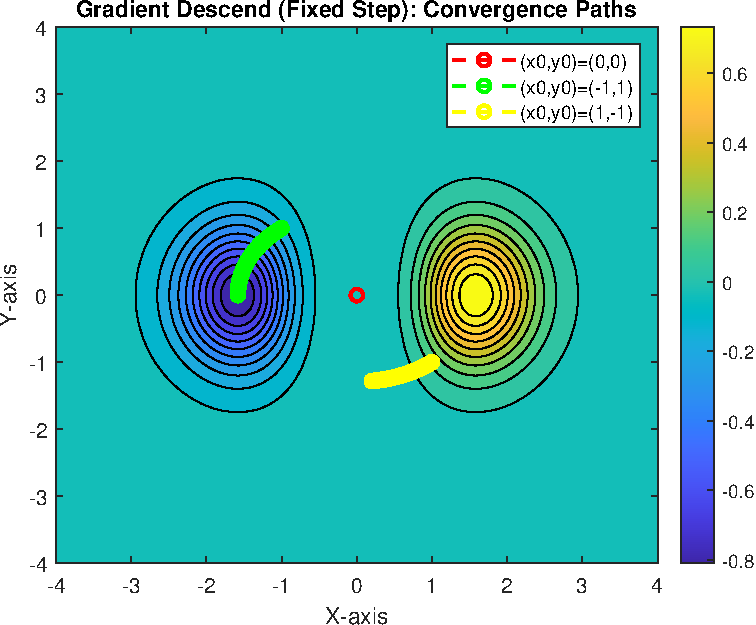
\includegraphics[width=1\linewidth]{plot/gradient_descend_fixed_step_contour.pdf}
        \caption{\small Διαδοχικά σημεία υπολογισμού της μεθόδου Μέγιστης Καθόδου για σταθερό βήμα $\gamma_k=0.001$}
        \label{fig:gradient_descend_fixed_step_contour}
    \end{minipage} \hfill
    \begin{minipage}{0.47\textwidth} % Ορίζει το πλάτος της δεύτερης εικόνας
        \centering
        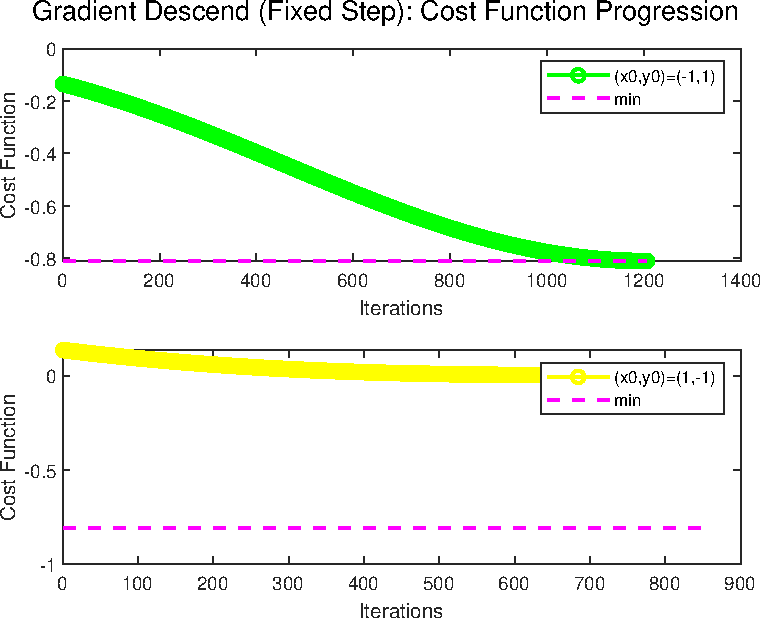
\includegraphics[width=1\linewidth]{plot/gradient_descend_fixed_step_costs.pdf}
        \caption{\small Σύγκλιση της μεθόδου Μέγιστης Καθόδου για σταθερό βήμα $\gamma_k=0.001$}
        \label{fig:gradient_descend_fixed_step_costs}
    \end{minipage}
\end{figure}

\subsection*{Βήμα με ελαχιστοποίηση}
Σε αυτή την περίπτωση θα υπολογίσουμε το $\gamma_k$ που ελαχιστοποιεί την $f(x_k + \gamma_k d_k)$ σε ένα προκαθορισμένο
διάστημα αναζήτησης $d$. Για τον σκοπό αυτό θα χρησιμοποιήσουμε την μέθοδο \selectlanguage{english} Fibonacci.
\selectlanguage{greek} Πρόφανώς για να συγκλίνει η μέθοδος \selectlanguage{english} Fibonacci \selectlanguage{greek} 
στο ελάχιστο θα πρέπει η συνάρτηση να είναι αυστηρά σχεδόν κυρτή στο $d$. Επίσης για το αρχικό σημείο $(1, -1)$, 
το $d$ πρέπει να είναι αρκούντως μεγάλο ώστε να ξεπεράσουμε την περιοχή όπου $\nabla f \approx 0$. Στο 
Σχήμα~\ref{fig:gradient_descend_line_minimization_contour}
παρατηρούμε ότι η μέθοδος συγκλίνει για τα αρχικά σημεία $(-1, 1)$, $(1, -1)$. Επίσης βλέπουμε ότι η πορεία προς το 
ελάχιστο είναι μία τεθλασμένη γραμμή, με τα διαδοχικά ευθύγραμμα τμήματα να είναι κάθετα μεταξύ τους, όπως αναμέναμε
άλωστε από την θεωρία. Από το Σχήμα~\ref{fig:gradient_descend_line_minimization_costs} φαίνεται πως η σύγκλιση για 
αρχικό σημείο $(-1, 1)$ επιτεύθχει με πολύ μικρότερο αριθμό επαναλήψεων από ότι στην περίπτωση του σταθερού βήματος.

\begin{figure}[h]
    \centering
    \begin{minipage}{0.47\textwidth}
        \centering
        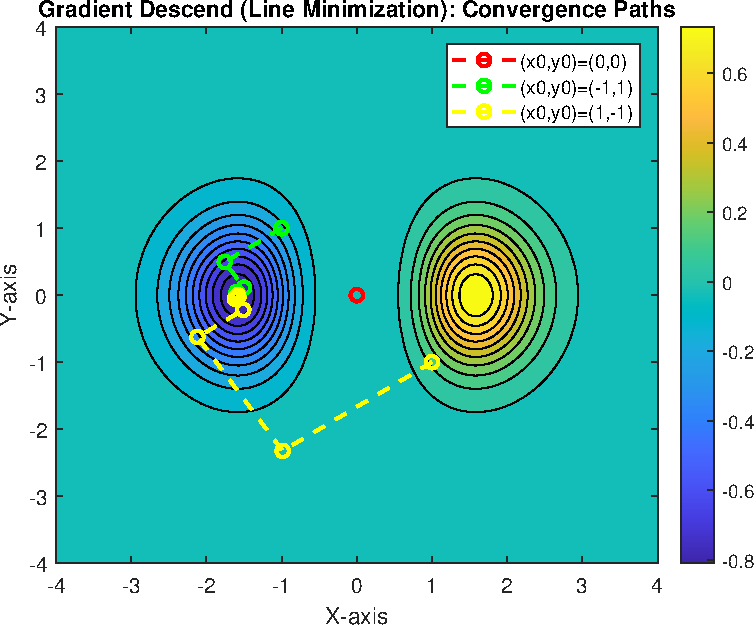
\includegraphics[width=1\linewidth]{plot/gradient_descend_line_minimization_contour.pdf}
        \caption{\small Διαδοχικά σημεία υπολογισμού της μεθόδου Μέγιστης Καθόδου για βήμα μέσω ελαχιστοποίησης}
        \label{fig:gradient_descend_line_minimization_contour}
    \end{minipage} \hfill
    \begin{minipage}{0.47\textwidth}
        \centering
        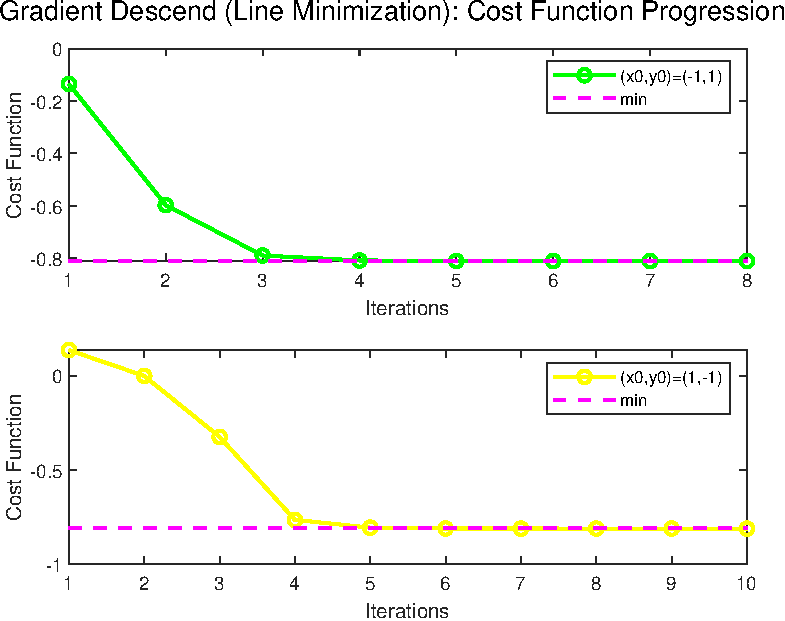
\includegraphics[width=1\linewidth]{plot/gradient_descend_line_minimization_costs.pdf}
        \caption{\small Σύγκλιση της μεθόδου Μέγιστης Καθόδου για βήμα μέσω ελαχιστοποίησης}
        \label{fig:gradient_descend_line_minimization_costs}
    \end{minipage}
\end{figure}

\subsection*{Βήμα με τον κανόνα \selectlanguage{english} Armijo}
\selectlanguage{greek}
Στο Σχήμα~\ref{fig:gradient_descend_armijo_rule_iters} βλέπουμε τις τρεις πρώτες επαναλήψεις της μεθόδου
\selectlanguage{english} Armijo \selectlanguage{greek} για τα αρχικά σημεία $(-1, 1)$, $(1, -1)$ για
$s = 3$, $\beta = 0.5$ και $\alpha = 0.01$. Όπως και στην περίπτωση της ελαχιστοπόιησης, το αρχικό βήμα $s$
πρέπει να είναι αρκούντως μεγάλο ώστε να ξεπεράσουμε την περιοχή όπου $\nabla f \approx 0$ και να έχουμε σύγκλιση
του $(1, -1)$. Από το Σχήμα~\ref{fig:gradient_descend_armijo_rule_costs} βλέπουμε ότι η μέθοδος μέγιστης καθόδου
με τον κανόνα \selectlanguage{english} Armijo \selectlanguage{greek} απαιτεί περίπου τον ίδιο αριθμό επαναλήψεων
με αυτόν της ελαχιστοποίησης συνάρτησης.

\begin{figure}
    \centering
    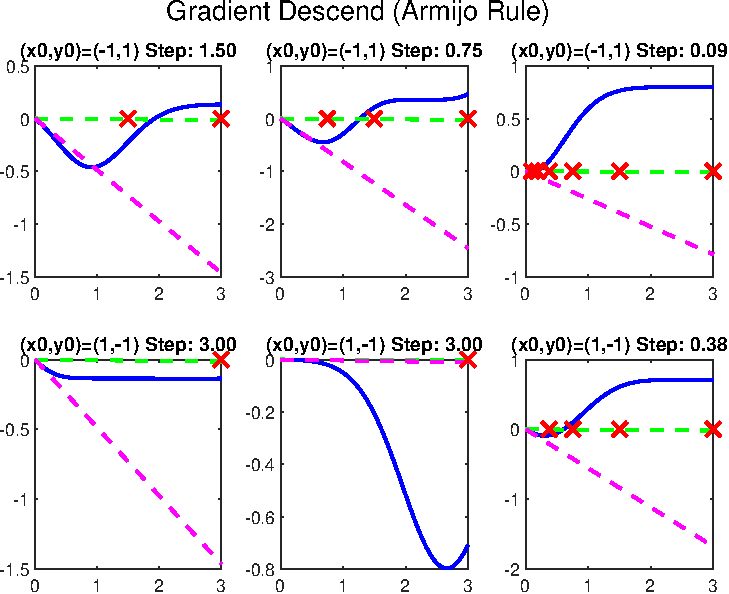
\includegraphics[width=1\linewidth]{plot/gradient_descend_armijo_rule_iters.pdf}
    \caption{Μέθοδος \selectlanguage{english} Armijo \selectlanguage{greek} για τις τρεις πρώτες επαναλήψεις της μεθόδου Μέγιστης Καθόδου}
    \label{fig:gradient_descend_armijo_rule_iters}
\end{figure}

\begin{figure}[h]
    \centering
    \begin{minipage}{0.47\textwidth}
        \centering
        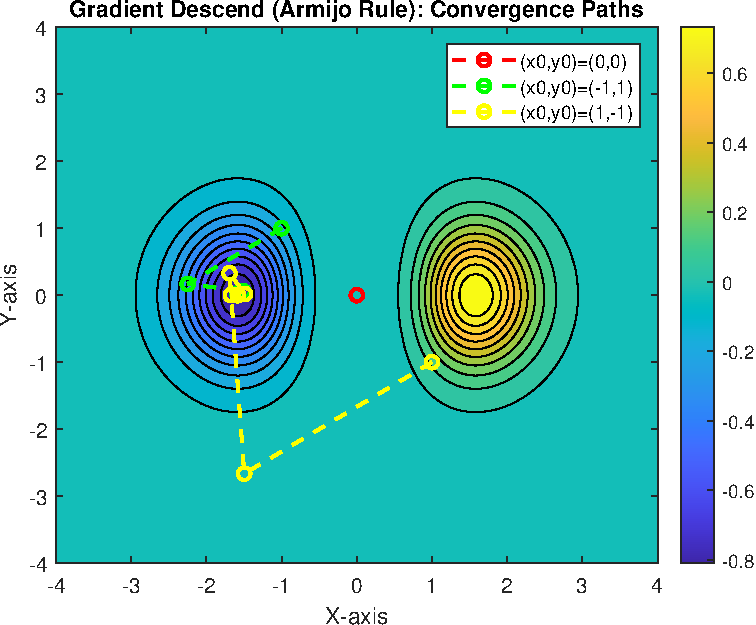
\includegraphics[width=1\linewidth]{plot/gradient_descend_armijo_rule_contour.pdf}
        \caption{\small Διαδοχικά σημεία υπολογισμού της μεθόδου Μέγιστης Καθόδου για βήμα μέσω του κανόνα \selectlanguage{english} Armijo \selectlanguage{greek}}
        \label{fig:gradient_descend_armijo_rule_contour}
    \end{minipage} \hfill
    \begin{minipage}{0.47\textwidth}
        \centering
        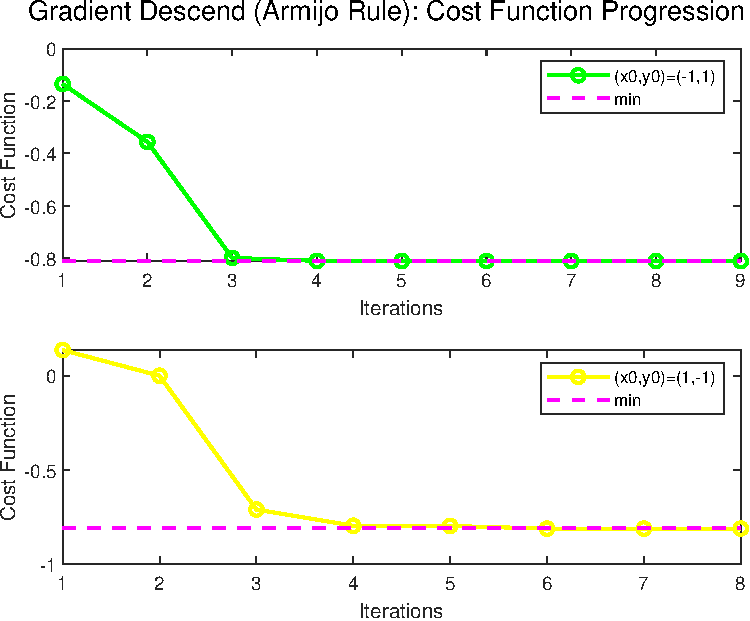
\includegraphics[width=1\linewidth]{plot/gradient_descend_armijo_rule_costs.pdf}
        \caption{\small Σύγκλιση της μεθόδου Μέγιστης Καθόδου για βήμα μέσω του κανόνα \selectlanguage{english} Armijo \selectlanguage{greek}}
        \label{fig:gradient_descend_armijo_rule_costs}
    \end{minipage}
\end{figure}


\section*{Μέθοδος \selectlanguage{english} Newton}
Σε αυτή τη μέθοδο, το διάνυσμα κατεύθυνσης $d_k$ επιλέγεται ως 
\[d_k = -\frac{[\nabla^2 f(x_k)]^{-1} \nabla f(x_k)}{|[\nabla^2 f(x_k)]^{-1} \nabla f(x_k)|}\]
όπου $\nabla^2 f(x_k)$ ο εσσιανός πίνακας της αντικειμενικής συνάρτησης. Η κανονικοποίηση του $d_k$ 
γίνεται για τους λόγους που αναφέρθηκαν παραπάνω. Επειδή η συγκεκριμένη μέθοδος λαμβάνει υπ' όψιν
την κυρτότητα της συνάρτησης επιτυγχάνει ταχύτερη σύγκλιση σε σχέση με την μέθοδο της μέγιστης καθόδου.
Ωστόσο αυτή η επιτάχυνση έρχεται και με μεγαλύτερο υπολογιστικό κόστος λόγω του υπολογισμού του αντίστροφου
του εσσιανού πίνακα. Ένα άλλο μειονέκτημα της μεθόδου είναι η απαίτηση ο εσσιανος πίνακας να είναι θετικά 
ορισμένος ώστε να μπορέσει να συγκλίνει στο ολικό ελάχιστο. Αυτός είναι και ο λόγος που στην περίπτωσή μας
ο αλγόριθμος αποτυγχάνει για τα αρχικά σημεία $(-1, 1)$, $(1, -1)$. Στο Σχήμα~\ref{fig:newton_fixed_step_contour}
έως Σχήμα~\ref{fig:newton_armijo_rule_costs} φαίνεται η απόκλιση του αλγορίθμου για κάθε περίπτωση υπολογισμού
του βήματος.

\begin{figure}[h]
    \centering
    \begin{minipage}{0.47\textwidth}
        \centering
        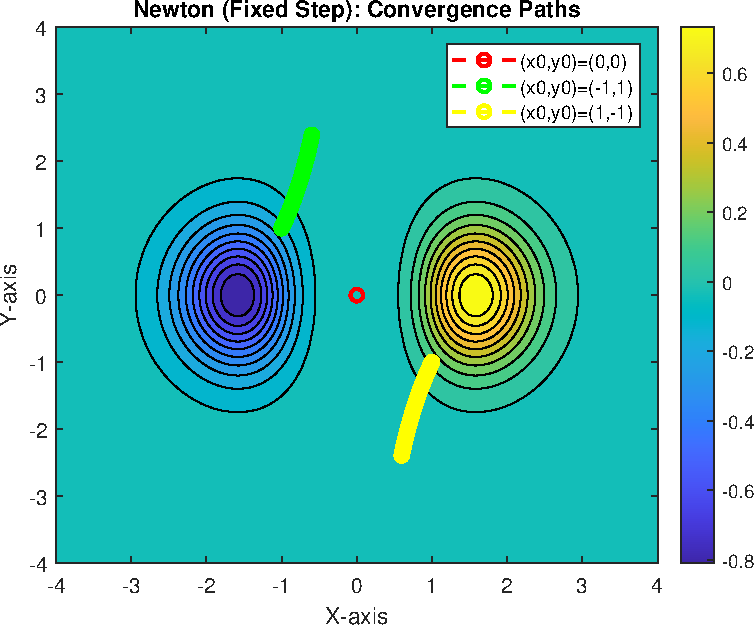
\includegraphics[width=1\linewidth]{plot/newton_fixed_step_contour.pdf}
        \caption{\small Διαδοχικά σημεία υπολογισμού της μεθόδου \selectlanguage{english} Newton \selectlanguage{greek} για σταθερό βήμα}
        \label{fig:newton_fixed_step_contour}
    \end{minipage} \hfill
    \begin{minipage}{0.47\textwidth}
        \centering
        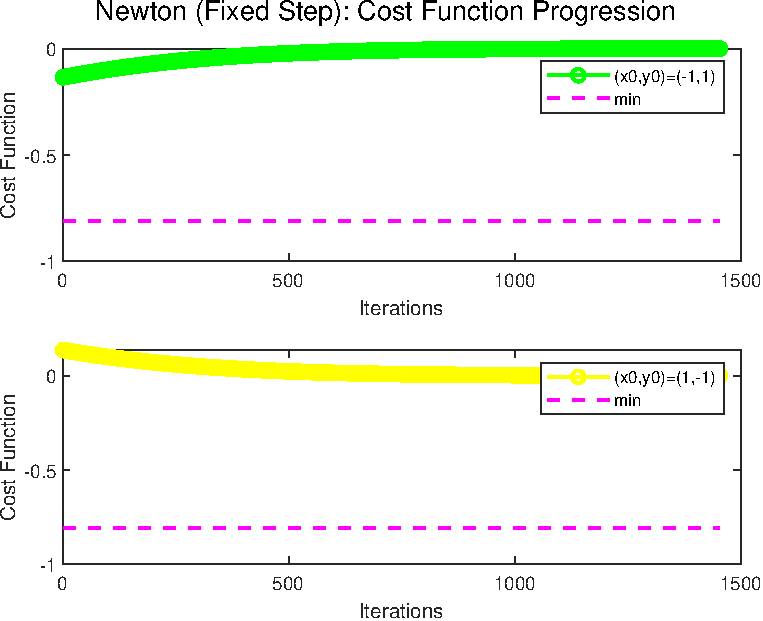
\includegraphics[width=1\linewidth]{plot/newton_fixed_step_costs.pdf}
        \caption{\small Σύγκλιση της μεθόδου \selectlanguage{english} Newton \selectlanguage{greek} για σταθερό βήμα}
        \label{fig:newton_fixed_step_costs}
    \end{minipage}
\end{figure}

\begin{figure}[h]
    \centering
    \begin{minipage}{0.47\textwidth}
        \centering
        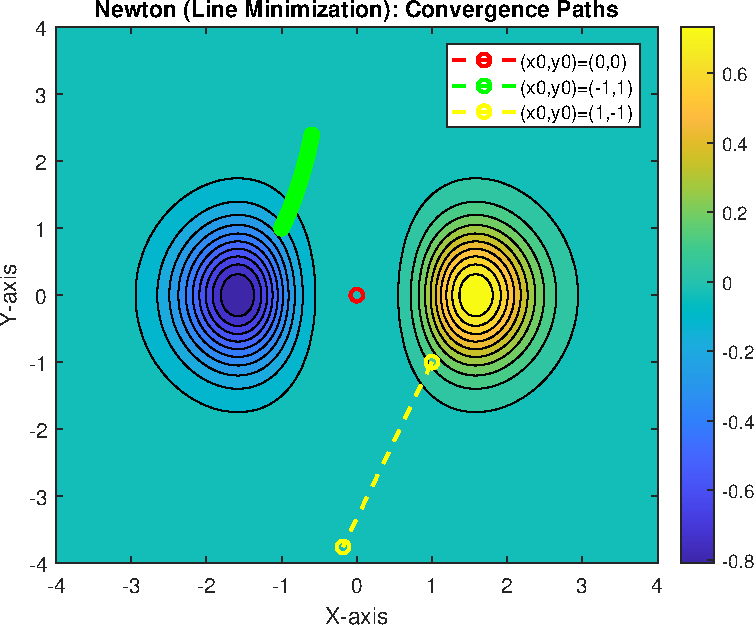
\includegraphics[width=1\linewidth]{plot/newton_line_minimization_contour.pdf}
        \caption{\small Διαδοχικά σημεία υπολογισμού της μεθόδου \selectlanguage{english} Newton \selectlanguage{greek} για βήμα μέσω ελαχιστοποίησης}
        \label{fig:newton_line_minimization_contour}
    \end{minipage} \hfill
    \begin{minipage}{0.47\textwidth}
        \centering
        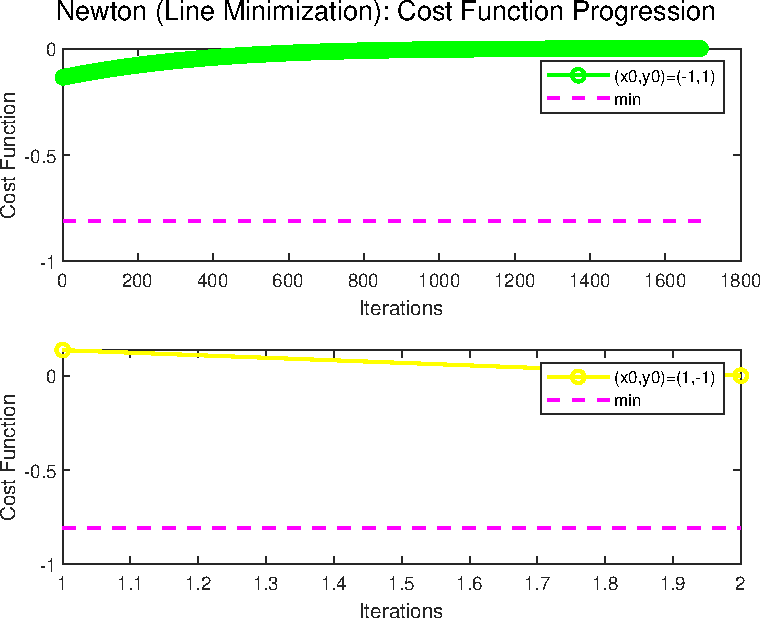
\includegraphics[width=1\linewidth]{plot/newton_line_minimization_costs.pdf}
        \caption{\small Σύγκλιση της μεθόδου \selectlanguage{english} Newton \selectlanguage{greek} για βήμα μέσω ελαχιστοποίησης}
        \label{fig:newton_line_minimization_costs}
    \end{minipage}
\end{figure}

\begin{figure}[h]
    \centering
    \begin{minipage}{0.47\textwidth}
        \centering
        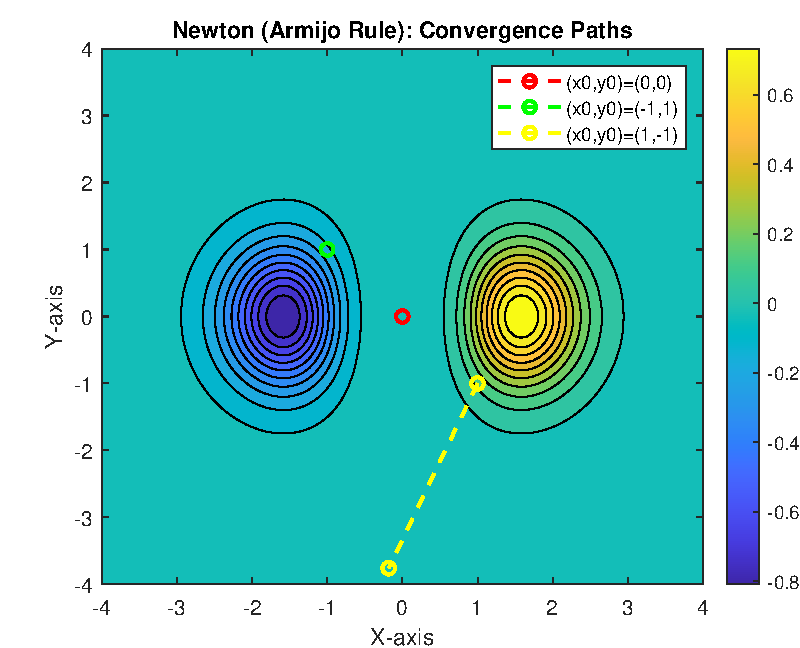
\includegraphics[width=1\linewidth]{plot/newton_armijo_rule_contour.pdf}
        \caption{\small Διαδοχικά σημεία υπολογισμού της μεθόδου \selectlanguage{english} Newton \selectlanguage{greek} για βήμα μέσω του κανόνα \selectlanguage{english} Armijo \selectlanguage{greek}}
        \label{fig:newton_armijo_rule_contour}
    \end{minipage} \hfill
    \begin{minipage}{0.47\textwidth}
        \centering
        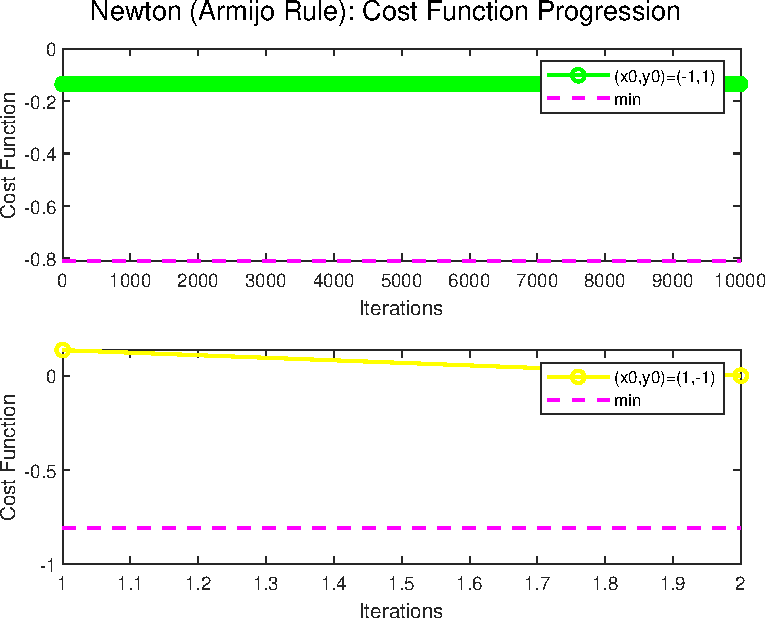
\includegraphics[width=1\linewidth]{plot/newton_armijo_rule_costs.pdf}
        \caption{\small Σύγκλιση της μεθόδου \selectlanguage{english} Newton \selectlanguage{greek} για βήμα μέσω του κανόνα \selectlanguage{english} Armijo \selectlanguage{greek}}
        \label{fig:newton_armijo_rule_costs}
    \end{minipage}
\end{figure}

\section*{Μέθοδος \selectlanguage{english} Levenberg-Marquardt}


\section*{Συμπέρασμα}



\end{document}
